% !TEX root = ../main.tex
\subsubsection{FMT Reconstruction}
\label{sssec::fmt_reconstruction}
    \begin{wrapfigure}{r}{0.50\textwidth}
        \centering\frame{
        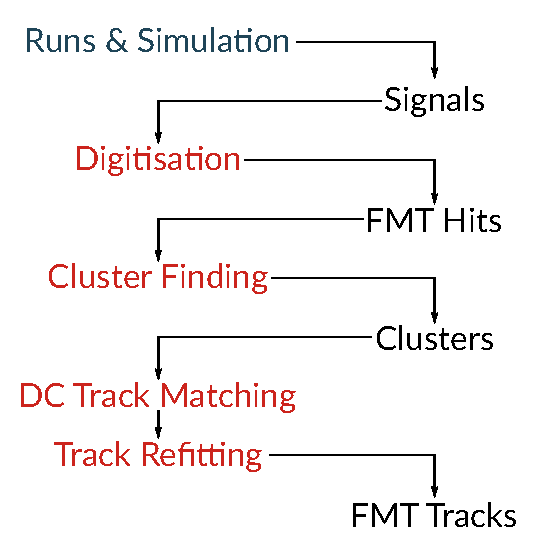
\includegraphics[width=\linewidth]{10fmt_recon.pdf}}
        \caption[FMT reconstruction summary]{FMT reconstruction summary.
        Data taking is coloured blue, data in black, and processes in red.
        Source: Own elaboration using \hyperlink{inkscape.org/}{Inkscape}.}
        \label{fig::fmt_recon}
    \end{wrapfigure}

    Once a signal is detected on a readout strip and the data is stored, the information is extracted from it during offline reconstruction.
    The reconstruction process of the FMT closely resembles that of the DC.

    To begin with, when a signal is detected in a strip, it undergoes digitization, processing, and is transformed into an \textbf{FMT Hit}.
    A set of FMT hits is then processed using a \textbf{Cluster Finding} algorithm, where a \textbf{Cluster} is defined as a group of hits that likely originate from the same particle track.
    Groups of clusters from different layers are subjected to a \textbf{DC Track Matching} algorithm, where they are matched to DC tracks generated by the DC Reconstruction process.
    Subsequently, a \textbf{Track Refitting} algorithm is employed for each DC track using the data from the clusters, resulting in updated tracks known as \textbf{FMT tracks}.
    An overview of this entire process is provided in figure \ref{fig::fmt_recon}.

    \clearpage
